\slajdid{07-s005}
\begin{frame}[label=07-s005]{Primer i ideja jedne programabilne komponente}
\gusttekst\centering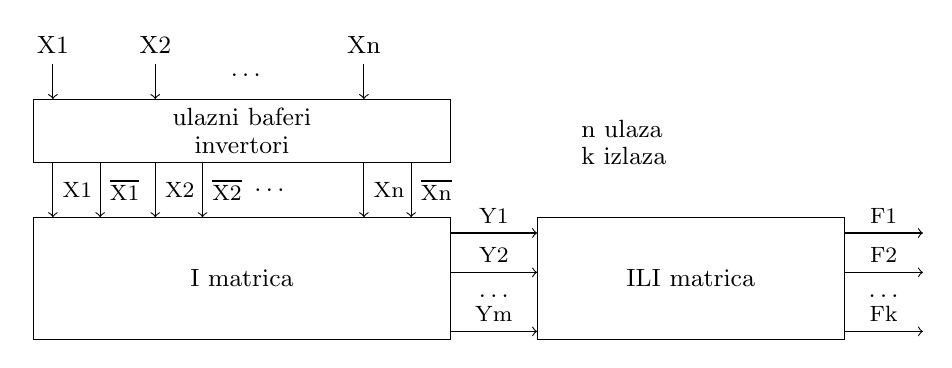
\begin{tikzpicture}[x=1cm,y=1cm,font=\fontsize{9}{10}\selectfont]
\draw (0,2.25) rectangle (5.3,3.05);\node[align=center] at (2.65,2.65) {ulazni baferi\\invertori};
\draw (0,0) rectangle (5.3,1.55);\node at (2.65,.775) {I matrica};
\draw (6.4,0) rectangle (10.3,1.55);\node at (8.35,.775) {ILI matrica};
\node[align=left] at (7.5,2.5) {n ulaza\\k izlaza};
\draw[->] (0.25,3.5) node[above] {X1}--(0.25,3.05);
\draw[->] (1.55,3.5) node[above] {X2}--(1.55,3.05);
\draw[->] (4.2,3.5) node[above] {Xn}--(4.2,3.05);
\node at (2.7,3.35) {$\ldots$};
\node at (3,1.9) {$\ldots$};
\draw[->] (0.25,2.25)--(0.25,1.55) node[midway,right=0pt,font=\fontsize{8}{9}\selectfont] {X1};
\draw[->] (0.85,2.25)--(0.85,1.55) node[midway,right=0pt,font=\fontsize{8}{9}\selectfont] {$\overline{\mathrm{X1}}$};
\draw[->] (1.55,2.25)--(1.55,1.55) node[midway,right=0pt,font=\fontsize{8}{9}\selectfont] {X2};
\draw[->] (2.15,2.25)--(2.15,1.55) node[midway,right=0pt,font=\fontsize{8}{9}\selectfont] {$\overline{\mathrm{X2}}$};
\draw[->] (4.2,2.25)--(4.2,1.55) node[midway,right=0pt,font=\fontsize{8}{9}\selectfont] {Xn};
\draw[->] (4.8,2.25)--(4.8,1.55) node[midway,right=0pt,font=\fontsize{8}{9}\selectfont] {$\overline{\mathrm{Xn}}$};
\draw[->] (5.3,1.35)--(6.4,1.35) node[midway,above=0pt,font=\fontsize{8}{9}\selectfont] {Y1};
\draw[->] (10.3,1.35)--(11.3,1.35) node[midway,above=0pt,font=\fontsize{8}{9}\selectfont] {F1};
\draw[->] (5.3,0.85)--(6.4,0.85) node[midway,above=0pt,font=\fontsize{8}{9}\selectfont] {Y2};
\draw[->] (10.3,0.85)--(11.3,0.85) node[midway,above=0pt,font=\fontsize{8}{9}\selectfont] {F2};
\draw[->] (5.3,0.1)--(6.4,0.1) node[midway,above=0pt,font=\fontsize{8}{9}\selectfont] {Ym};
\draw[->] (10.3,0.1)--(11.3,0.1) node[midway,above=0pt,font=\fontsize{8}{9}\selectfont] {Fk};
\node at (5.85,.55) {$\ldots$};\node at (10.8,.55) {$\ldots$};
\end{tikzpicture}
\par\vspace{2mm}
\raggedright Šta i koliko može da se programira zavisi od tipa komponente.\par\vspace{2mm}
Da li su obe matrice programabilne?\\
Da li je samo I odnosno ILI matrica programabilna?\\
Koliko su programabilne?\\
Šta može da učestvuje u Y i koliko ih ima (m?)? Koliko ulaza u I kola.\\
Šta može da učestvuje u F i koliko? Koliko ulaza u ILI kola.
\end{frame}
